\documentclass[aspectratio=169]{beamer}
\usetheme{Madrid}
\usecolortheme{beaver}
\usepackage[utf8]{inputenc}
\usepackage[T1]{fontenc}
\usepackage{tikz}
\usepackage{amssymb}
\usepackage{graphicx}
\setbeamertemplate{navigation symbols}{}
\setbeamercolor{title}{fg=white,bg=cyan!60!black}
\setbeamercolor{frametitle}{fg=white,bg=cyan!50!black}
\setbeamercolor{block title}{bg=cyan!15,fg=black}
\setbeamercolor{block body}{bg=cyan!5,fg=black}

\title{G9 — Strings \& Dialogue}
\subtitle{Lesson 2: Dialogue Tree}
\author{ByteForge --- Grade 7 --- Game Maker}
\date{}

\begin{document}

\begin{frame}
    \titlepage
\end{frame}

\begin{frame}{Comparing text to branch a conversation}
    \Large
    \texttt{===} works on text just like on numbers — the entire mechanism behind a dialogue tree: compare a choice, branch to different text.

    \begin{center}
    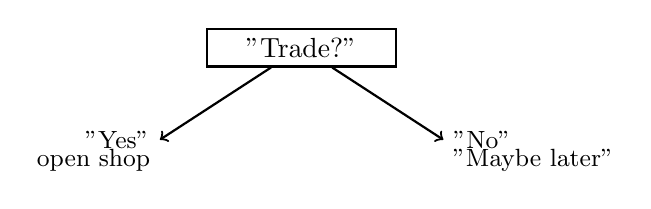
\begin{tikzpicture}[scale=0.9]

        \node[draw, thick, minimum width=2.4cm] (a) at (0,0) {"Trade?"};
        \draw[->, thick] (a) -- (-2,-1.3) node[left]{\small "Yes"};
        \draw[->, thick] (a) -- (2,-1.3) node[right]{\small "No"};
        \node[below left] at (-2,-1.3) {\small open shop};
        \node[below right] at (2,-1.3) {\small "Maybe later"};
    \end{tikzpicture}
    \end{center}
\end{frame}

\begin{frame}{Your Turn}
    \Large
    Open the student map, find \textbf{G9 — Strings \& Dialogue}, and complete
    the \textbf{Dialogue Tree} challenge --- everything you just saw, they now do themselves.
\end{frame}

\end{document}
